%%%%%%%%%%%%%%%%%%%%%%%%%%%%%%%%%%%%%%%%%%%%%%%%%
%
% Universita' degli Studi dell'Insubria
% Template LaTeX realizzato da Nicola Landro
%
%%%%%%%%%%%%%%%%%%%%%%%%%%%%%%%%%%%%%%%%%%%%%%%%%
\documentclass[a4paper, 11pt, twoside]{book} % twoside, oneside
\usepackage[a4paper]{geometry}
\usepackage[italian]{babel}
\usepackage{textcomp}
\usepackage{color}
\usepackage{url}
\usepackage{amsfonts}
\usepackage{float}
\usepackage{booktabs}
\usepackage{longtable}
\usepackage{makeidx}
\usepackage{fancyhdr}
\usepackage[times]{quotchap}
\usepackage{multirow}
\usepackage{version}

\usepackage{listings}
\usepackage{color}
\definecolor{gray}{rgb}{0.9,0.9,0.9}
\definecolor{orange}{rgb}{0.9,0.5,0.08}
\definecolor{purple}{rgb}{0.5,0.01,0.5}


%%Stile per codice

\lstdefinestyle{customjava}{
  	language=Java,
  	frame=tlrb,
  	aboveskip=3mm,
  	belowskip=6mm,
  	showstringspaces=false,
  	columns=flexible,
  	basicstyle={\small\ttfamily},
  	numbers=left,
    numberstyle=\tiny\color{orange}\ttfamily,
    numbersep=5pt,
  	keywordstyle=\color{purple},
  	commentstyle=\color{orange},
  	stringstyle=\color{blue},
  	breaklines=true,
  	breakatwhitespace=true
  	tabsize=3
}


%% Aggiunge una linea al di sotto di ogni sezione principale
\usepackage[calcwidth]{titlesec}
\titleformat{\section}[hang]{\sffamily\bfseries}
 {\Large\thesection}{12pt}{\Large}[{\titlerule[0.4pt]}]

%% Gestisce la grafica a seconda che si usi latex o pdflatex
\newif\ifpdf
\ifx\pdfoutput\undefined
\pdffalse % no pdflatex
\else
\pdfoutput=1 % pdflatex
\pdftrue
\fi
%
\ifpdf
\usepackage[pdftex]{floatflt,graphicx}
\DeclareGraphicsExtensions{.pdf,.mps,.png,.jpg}
\usepackage[pdftex]{hyperref}
\else
\usepackage{floatflt,graphicx}
\DeclareGraphicsExtensions{.eps}
\fi
\usepackage{subfigure}

%\usepackage{algorithm}
%\usepackage{algorithmic}
\usepackage[utf8]{inputenc} % per accenti

%%tabella con linee colorate
\usepackage{colortbl}

%%%%%%%%%%%%% NUOVI COMANDI E IMPOSTAZIONI %%%%%%%%%%%
\newenvironment{mcquote}
  {\begin{list}{}{
      \setlength{\rightmargin}{\leftmargin}}
         \item[]``\ignorespaces}
  {\unskip''\end{list}}
  
\newcommand{\mcchap}[2]{\protect{
 \chapter{#1}
 \label{#2}
}}

%% Gestione header: no header sulle dispari bianche
\makeatletter
\def\cleardoublepage{\clearpage\if@twoside \ifodd\c@page\else%
    \hbox{}%
    \thispagestyle{empty}%              % Empty header styles
    \newpage%
    \if@twocolumn\hbox{}\newpage\fi\fi\fi}
\makeatother

\newcommand{\codice}[1]{\protect\texttt{\small{#1}}}

\newcommand{\mcproc}[1]{\ensuremath{\mbox{\sc #1}}}

\newcommand{\mctodo}[1]{\protect{
  \bigskip
  \begin{tabular}{|p{13cm}} \textcolor{red}{\underline{TODO:}} \small{#1} \end{tabular}}
}

\newcommand{\mcnota}[1]{\protect{
  \bigskip
  \begin{tabular}{|p{13cm}} \underline{NOTA:} \small{#1} \end{tabular}}
}

\makeindex
\linespread{1.1}
%\floatname{algorithm}{Algoritmo}
%\renewcommand{\listalgorithmname}{Elenco degli algiritmi}



%%%%%%%%%%%%%%%% METADATI DOCUMENTO %%%%%%%%%%%%%%%%%%
\date{}

%%%%%%%%%%%%%%%%%% INIZIO DOCUMENTO %%%%%%%%%%%%%%%%%%
\begin{document}
\pagestyle{empty}

%% Pagina del titolo
  \begin{titlepage}
  \begin{center}
  \begin{large}
  {\fontsize{20.74}{18}\selectfont\vspace*{0.50cm}Universit\`a degli Studi dell'Insubria}\\
  Facolt\`a di Scienze MM.FF.NN.\\
  Corso di Laurea Triennale in Informatica
  \end{large}
  
  \vspace{1cm}
  \begin{figure}[h]
    \begin{center}
      
\includegraphics[scale=0.25]{copertina/logounivector.pdf}
    \end{center}
  \end{figure}

    {\fontsize{26}{26}\usefont{OT1}{phv}{m}{n}\selectfont\par\vspace*{0.75cm}
    Ristutturazione di un sistema
    \vspace{.15em}di gestione dei contenuti}
    \par
    
    \vfill
    \vspace{3cm}
    \begin{large}
    Relatore: Dott. Ignazio Gallo\\

    \vspace{1.0cm}
    Tesi di Laurea di\\
   Matteo Franceschi De Marchi\\
    Matricola 325680\\
    \vspace{0.5cm}

    \end{large}

    Anno Accademico 2016-2017

  \end{center}
\end{titlepage}


%% Dedica
\frontmatter{}
  \begin{flushright}
    \vspace*{0cm}
    \vfill
    \textit{ 
      ``What a liberation to realize that the “voice in my head” is not who I am. Who am I then? The one who sees that.''- Eckhart Tolle
    }
    \vspace{2.5cm}
  \end{flushright}
  \cleardoublepage
  
%% Indice ed elenchi
  
  \pagenumbering{roman}
  \setcounter{page}{1}
  \setcounter{tocdepth}{2}
  \tableofcontents
  \listoffigures
  \listoftables
%% Inizio capitoli
  \mainmatter{}
  
%% Capitoli
  \pagestyle{fancy}
  \renewcommand{\chaptermark}[1]{\markboth{#1}{}} 
  \renewcommand{\sectionmark}[1]{\markright{\thesection\ #1}} 
  \fancyhf{} % delete current setting for header and footer 
  \fancyhead[LE,RO]{\bfseries\thepage} 
  \fancyhead[LO]{\bfseries\rightmark} 
  \fancyhead[RE]{\bfseries\leftmark} 
  \renewcommand{\headrulewidth}{0.8pt} 
  \renewcommand{\footrulewidth}{0pt} 
  %\renewcommand{\headheight}{16pt}
  \addtolength{\headheight}{0.5pt} % make space for the rule 
  \fancypagestyle{plain}{% 
  \fancyhead{} % get rid of headers on plain pages
  \fancyfoot[C]{\bfseries \thepage}
  \renewcommand{\headrulewidth}{0pt} % and the line 
  } 

  \cleardoublepage{}
  \setcounter{page}{1}
  
%-------------------------------------------------------------
%				INTRODUZIONE
%-------------------------------------------------------------

\mcchap{Introduzione}{cap:intro}

Nel periodo di apprendistato in 7Pixel sono stato assegnato al team Iguana, team che si occupa
della gestione principalmente front-end dei siti del \emph{Kirivo Network}

\section{Il Kirivo Network}
Il Kirivo Network (KN) è attualmente composto da due siti  \url{www.kirivo.it} 
e \url{www.origini.it}:

\url{www.kirivo.it} è un negozio online che vende prodotti di tutte le categorie.
Il marketplace dispone di un offerta di oltre 800.000 articoli in tutte le categorie tra cui
elettrodomestici, prodotti per la casa, smartphone e TV, giocattoli, moda e altri.

\url{www.kirivo.it} è il marketplace ufficiale di \url{www.trovaprezzi.it}, il principale motore
di ricerca italiano per la comparazione di prezzi.

\url{www.origini.it} è una divisione verticale di Kirivo. Il sito è specializzato nella vendita
di vini e offre un ampia offerta di prodotti divisi per cantine e regioni. Il sito
è online da Novembre 2016.

I siti del Kirivo Network fanno utilizzo di servizi di Back-End comuni che permettono 
di effettuare acquisti nei due siti utilizzando un unico account ed un unico carrello.

Con buone probabilità verranno aggiunti in futuro nuovi siti verticali per alcune categorie
di Kirivo.

\section{Architettura del Kirivo Network}
Per l'erogazione dei siti del Kirivo network vengono usati diversi server:
\begin{itemize}
\item {\bf Hybris}: una piattaforma Enterprise di e-commerce scritta in Java che offre una soluzione all-in-one per i siti 
di e-commerce comprendendo servizi quali la gestione del catalogo dei prodotti, degli utenti e la 
gestione sicura dei pagamenti. La scelta di utilizzare una piattaforma di e-commerce a pagamento è stata fatta
principalmente per velocizzare i tempi di sviluppo in fase iniziale.

Hybris utilizza una database relazione Postgres e il suo cataologo viene indicizzato dal motore di ricerca SolR.

\item {\bf SolR}: un motore di ricerca scritto in Java che permette di indicizzare i prodotti presenti a catalogo per una accesso
più rapido.

Permette inoltre di filtrare in modo efficente i prodotti presenti a catalogo ottimizzando
le ricerche per categorie o caratteristiche del prodotto.

\item {\bf Kiruby}: un web-server Ruby che eroga le pagine web dei siti, si interfaccia con Hybris, Solr e Kitty utilizzando i loro
servizi di backend. 
\item {\bf Wordpress}: usato per la creazione di pagine di contenuto che vengono incluse da Kiruby.

Il server di Wordpress si trova nella LAN aziendale e si interfaccia solamente con il server Kiruby, la sua
presenza è nascosta agli utenti finali.
\item {\bf Redis}: un database noSql che, salvando tutto il suo contenuto in RAM, garantisce alte prestazioni.

Viene usato da Kiruby come cache di contenuti, specialmente per le richieste di Kiruby a Wordpress.

\item {\bf Nginx}: un Reverse proxy usato per redirigere le chiamate fatte ai domini \url{www.kirivo.it} 
e \url{www.origini.it} ai server opportuni.
\end{itemize}

\begin{figure}
  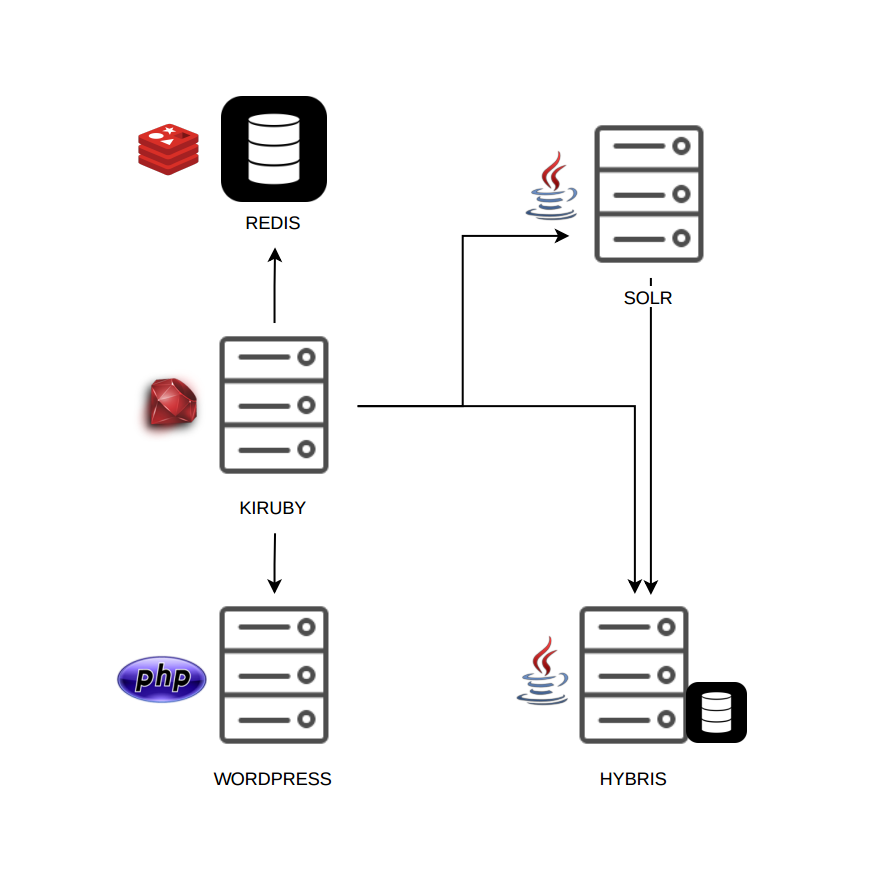
\includegraphics[width=\textwidth]{figure/arch.png}
  \caption{Schema dell'architettura del Kirivo Network.}
  \label{fig:kn}
\end{figure}


\newpage

\section{I team del Kirivo Network}
Lo sviluppo è l manutenzione dei siti del Kirivo Network viene effettuato da più team e questi sono:
\begin{itemize}
\item {\bf Team Iguana}: si occupano dello sviluppo di Kiruby.
\item {\bf Team Nimbus}: si occupano dello svliuppo di Hybris SolR e Kitty.
\item {\bf Content Manager}: si occupano della comunicazione con i venditori, della gestione dei prodotti a catologo
 e della creazione di pagine di speciali, lavorano interfacciandosi con Hybris e Wordpress.
\item {\bf Grafica}: lavora o direttamente su Kiruby o da al team Iguana grafiche HTML che vengono poi rese dinamiche 
ed integrate con i vari servizi.
\end{itemize}

\section{Gestione delle homepage} 	

Le homepage di Origini e Kirivo sono le pagine che, nei rispettivi siti, possono cambiare contenuto più 
frequentemente. Inoltre scegliere quali prodotti, quali offerte e quali contenuti 
vanno inseriti in homepage non è compito dei programmatori ma dei \emph{content managers},
quindi si rivela importante dare la possibilità ai \emph{content} di fare modifiche, come cambiare un prodotto da
mettere tra quelli in evidenza in homepage, o il testo di un pannello con la cantina del mese senza dover passare 
dai programmatori per fare modifiche.

Per dare più libertà ai \emph{content}, il contenuto della homepage, ovvero tutto quello che non è
header e footer, non si trova nel server Kiruby ma in pagine Wordpress che i content possono direttamente 
modificare accedendo alla sezione admin di Wordpress.

\begin{figure}
  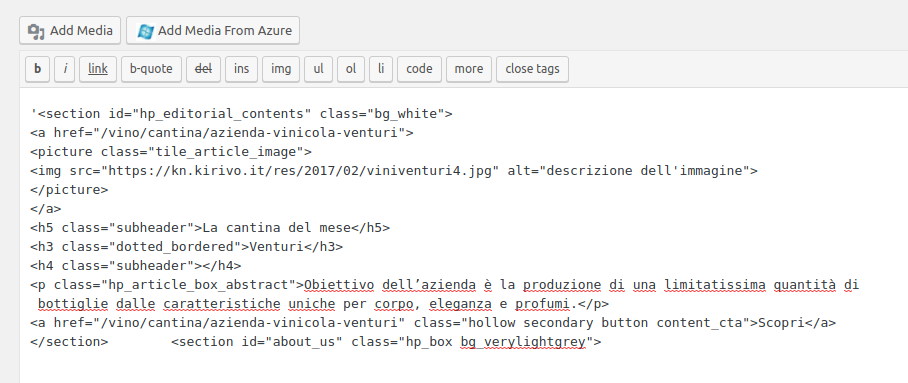
\includegraphics[width=\textwidth]{figure/whtml.png}
  \caption{L'interfaccia visualizzata dai content managers per modificare la pagina.}
  \label{fig:whtml}
\end{figure}

\begin{figure}
  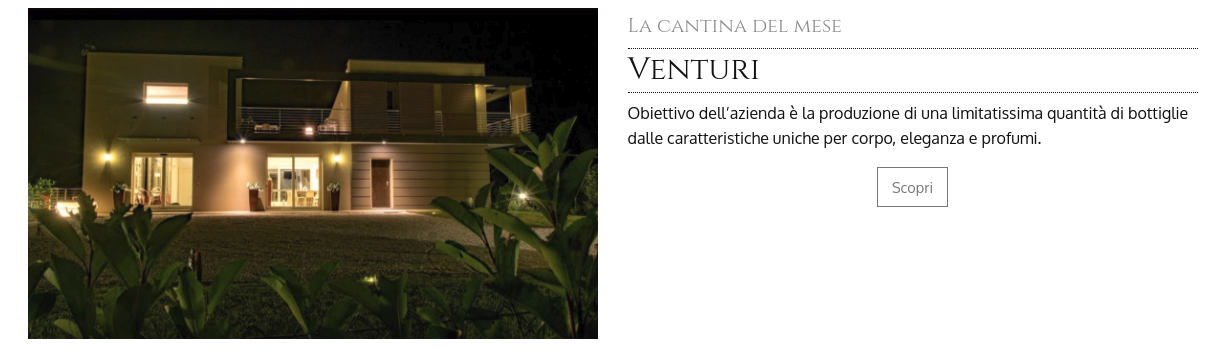
\includegraphics[width=\textwidth]{figure/wrender.png}
  \caption{Risultato renderizzato della componente compilata in figura \ref{fig:whtml}.}
  \label{fig:wrender}
\end{figure}


\newpage

Il server Kiruby quando deve riceve una richiesta per la homepage chiede a Wordpress la sua pagina della home, ne estrae
il contenuto e lo renderizza nell'HTML che restituisce. Il contenuto di Wordpress viene incluso nell'HTML tra Header e Footer il cui codice invece resta in Kiruby, in comune a tutte le altre pagine.


\begin{figure}
  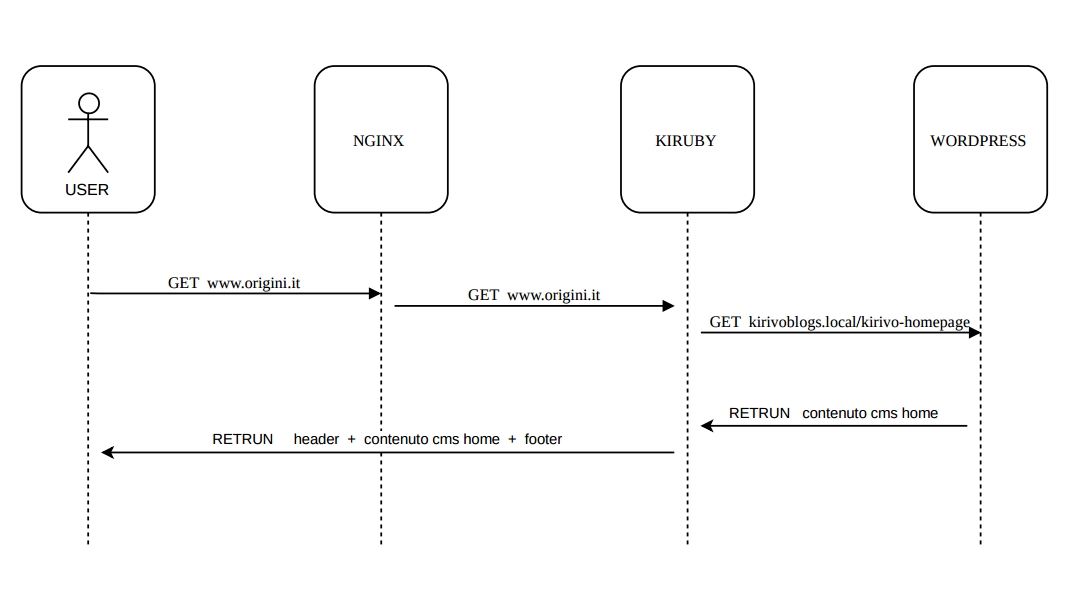
\includegraphics[width=\textwidth]{figure/homeseq.png}
  \caption{Funzionamento della richiesta della homepage.}
  \label{fig:homeseq}
\end{figure}



\section{La gemma cmsdealer}
Per visualizzare contenuti dinamici, come ad esempio un Box di 4 vini viene utilizzata
una gemma Ruby chiamata \emph{cmsdealer}.

La gemma è necessaria per il fatto che le informazioni dei prodotti non sono accessibili a Wordpress, che viene utilizzato
come server per la gestione e la modifica di contenuti editoriali, ma sono accessibili a Kiruby che ha al suo interno diversi
meccanismi per accedere alle informazioni dei prodotti andandosi ad interfacciare con Hybris e SolR.

La gemma \emph{cmsdealer} usata dal server Kiruby scansiona la pagina di Wordpress da includere,
se incontra un tag di nome \emph{dynamic} ne legge l'attributo \emph{type} e in base al valore di questo
seleziona il corrispondente template, legge l'ID dei prodotti e sostiusice al tag \emph{dyanmic} l'HTML del box con
i valori dei prodotti selezionati

Esempio: se processando la pagina HTML di Wordpress Kiruby trova
\begin{verbatim}
	<dynamic type="OriginiListingBox" ids="3422,2345,2872,2209" />
\end{verbatim}
allora verrà cercato il template di \emph{originilistingbox.html.erb} e verrà popolato
coi valori dei prodotti con gli identificativi specificati nell attributo \emph{ids}.

% immagine meta sito metà wp-admin di prodotti in evidenza

\newpage
\section{Obbiettivo}
L'obbiettivo del progetto è quello di rendere l'edit delle pagine
da parte dei content molto più semplice e flessibile,
facendo in modo che i contenuti delle homepage possano essere editati visualmente e non
andando a mettere mano direttamente sul codice HTML.

Per farlo i content dovranno interagire con un interfaccia grafica web che permette
la modifica delle informazioni necessarie e di poter spostare e copiare
componenti della home con un click o con un drag and drop.

\section{Obbiettivo secondario}
Obbiettivo secondario del progetto e di rendere il sito più manutenibile.

La criticità del sistema è che contiene codice duplicato nella gemma CmsDealer, in Kiruby
e nei widget di Wordpress. 

Per risolvere il problema sono state create le  \emph{RenderdPricesAPI} 
che restituiscono frammenti di HTML renderizzato per varie componenti della home.

In questo modo il codice del template resta solamente in Kiruby e esponendo le 
API questo viene usato sia dai Widget di Wordpress sia dalla gemma CmsDealer

  
%-------------------------------------------------------------
%				Studio in azienda
%-------------------------------------------------------------

\mcchap{Fase di formazione aziendale}{cap:agile}

Durante i primi due mesi di tirocinio, la maggior parte del mio tempo è stato speso in formazione,
l'obbiettivo dello studio era di fornirmi le conoscenze adeguate per lavorare nel progetto, in particolare lo studio
di Wordpress, e per integrarmi al Team Iguana per lo sviluppo e la manutenzione di Kiruby.


Il mio studio può essere diviso in tre argomenti principali:
\begin{itemize}
\item Ruby e le sue librerie
\item Wordpress
\item Sviluppo agile
\end{itemize}

Lo studio dei primi due è stato prevalentemente pratico, mentre lo studio e l'applicazione
delle metodologie agili è stato anche in buona parte teorico.

\section{Ruby e le sue librerie}

Il primo argomento di studio una volta entrato in azienda è stato il linguaggio \emph{Ruby}, essendo questo il
linguaggio del web server \emph{Kiruby} la quasi totalità del lavoro del mio Team viene svolto con questo linguaggio.

Per lo studio di Ruby mi sono affidato esclusivamente a risorse disponibili online, consigliate dal Team,
in particolare il sito \url{rubylearning.com}\cite{RUBY}.

In contemporanea a questo ho messo subito in pratica gli argomenti imparati risolvendo i \emph{Koans}\cite{KOANS}
di Ruby, ovvero una serie di test divisi per argomenti, come ad esempio String, Symbols, Hashes, Regular Expression, 
che inizialmente falliscono e che vanno sistemati in modo da passare correttamente. Quindi una volta studiato un certo argomento
veniva risolto il suo rispettivo \emph{Koan}. 

Una volta apprese le basi del linguaggio, per prendere maggiore confidenza ho iniziato a sviluppare
vari Kata agili.

I Kata agili sono dei programmi da sviluppare iterativamente, ovvero prima vengono fornite delle specifiche, una volta 
implementate se ne aggiungono di nuove o si modificano le precedenti. 

Questo tipo di esercizi serve a far abituare
lo svilppatore a scrivere codice in modo manutenibile, ovvero in modo che l'aggiunta o il cambiamento di una qualche 
funzionalità richieda il minimo sforzo grazie alla qualità del codice scritto.

Oltre alle basi del linguaggio ed ai Kata agili ho studiato anche l'utilizzo di alcune \emph{gemme} (così vengono chiamate le 
librerie Ruby) che vengono
usate frequentemente in Kiruby tra cui Test-Unit come framework di testing, librerie per l'integrazione
con SolR e Redis e librerie per lo scambio di dati JSON attraverso HTTP come \emph{HTTPParty}.

\section{Wordpress}

Parallelamente allo studio di Ruby mi sono dedicato allo studio di Wordpress.

Wordpress è il Content Managemente System più diffuso al mondo, è un applicazione web scritta in PHP
che deve essere servita da un web-server, solitamente Apache, nel nostro caso Nginx.

Nella fase di studio mi sono concentrato nell'analizzare e studiare come è struttrata l'applicazione
e dove un programmatore deve mettere mano per fare modifiche e personalizzare la propria installazione.

Oltre allo studio di Wordpress ho fatto un approfondimento del linguaggio PHP del quale avevo qualche
nozione ed esperienza di utilizzo, non troppo approfondita, già prima del mio arrivo. 




%-------------------------------------------------------------
%				AGILE
%-------------------------------------------------------------

\section{Sviluppo agile}

In 7Pixel si sviluppa utilizzando metodologie agili: il software viene sviuppato
iterativamente, nuove feature e aggiornamenti vengono pubblicati quotidianamente.
Nel periodo di studio le varie esercitazioni sono state effettuate
utilizzando due metodologie tipiche dello sviluppo agile.

\begin{itemize}
\item Test Driven Development
\item Pair Programming
\end{itemize}

\subsection{Test Driven Development}
Il TDD Test Driven Development è una tecnica utilizzata ovunque in azienda per lo sviluppo, nel TDD
prima di aggiungere una qualsiasi nuova funzionalità si scrive un test che passerebbe solo se 
quella funzionalità fosse implementata correttamente. 

Una volta scritto il test che fallisce, si cerca nel modo più veloce e semplice possibile di fare passare il test.

Una volta implementato il codice per far passare il test si fa del refactoring per rendere il codice più leggibile
e soprattutto manutenibile, cercando di eliminare il più possibile la presenza di codice duplicato.

\subsection{Pair Programming}
Pair Programming significa svilippo in coppia, ovvero due membri del Team lavorano contemporaneamente
allo stesso codice sulla stessa macchina, utilizzando due schermi speculari, due tastiere e due mouse

Il Pair Programming si rivela molto efficace, perchè si riescono ad evitare molti
errori di distrazione che possono costare caro in termini di tempo e soprattutto
si ha molto spesso la possibilità di confrontarsi con punti di vista diversi che possono
portare ad un analisi più approfondita del problema e a soluzioni migliori. 

Dal mio punto di vista di apprendista il Pair Programming ha portato inoltre il vantaggio
di poter lavorare con gente più esperta e quindi, durante il lavoro, di imparare tecniche,
metodologie e \emph{best pracitces} per lo sviluppo.

\subsection{Studio teorico}
Oltre alla messa in pratica delle tecniche di sviluppo agile sono stati anche effettuati studi teorici
su le come sviluppare codice pulito e manutenibile.

Gli argomenti principali sono stati:
\begin{itemize}
\item Studio dei principali design pattern, tra cui i pattern GRASP e SOLID.
\item Metodologie di refactoring.
\item Metodologie per mantenere il codice ordinato e leggibile.
\end{itemize}

  
%-------------------------------------------------------------
%				AGILE
%-------------------------------------------------------------

\mcchap{Sviluppo agile}{cap:agile}

In 7Pixel si sviluppo utilizzando metodologie agili, il software viene sviuppato
iterativamente, nuove feature e aggiornamenti vengono pubblicati quotidianamente.

\section{TDD}
Una tecnica rigorosamente usata in azienda è il TDD Test Driven Development ovvero, prima di
aggiungere una qualsiasi nuova funzionalità si scrive un test che passa solo se 
quella funzionalità fosse implementata. 

Dopodichè si cerca nel modo più veloce e semplice possibile di fare passare il test

Una volta passato il test si fa del refactoring per rendere il codice più leggibile
e soprattutto manutenibile

\section{Pair Programming}
Tutti i lavori effettuati su Kiruby sono sempre stati fatti in Pair Programming
con un membro del team

Il Pair Programming si rivela molto efficace, perchè si riescono ad evitare molti
errori "di distrazione" che possono costare caro in termini di tempo e soprattutto
si ha molto spesso la possibilità di confrontarsi con punti di vista diversi che possono
portare ad un analisi più approfondita del problema e a soluzioni migliori 


  
%-------------------------------------------------------------
%				Preparazione wordpress
%-------------------------------------------------------------

\mcchap{Preparazione dell'ambiente di sviluppo per Wordpress}{cap:Preparazione dell'ambiente di sviluppo}

Wordpress, essendo un Content Management System open source, è altamente personalizzabile e dispone
di un innumerevole quantità di \emph{plugin}, gratuiti e a pagamento, per ogni tipo di funzionalità.

Al mio arrivo veniva usata un'installazione base di Wordpress, con la sola aggiunta di un plugin chiamato \emph{Microsoft Azure 
for Wordpress} che fa in modo che tutte le immagini che vengono caricate dal pannello di admin di Wordpress
vengono caricate e servite da un server di Microsoft Azure.

Questo serve principalmente, come accennato precedentemente, ad oscurare il dominio del server di Wordpress,
infatti se in una pagina del KN fossero linkate le immagini con l'URL di Wordpress questo potrebbe 
comportare dei problemi di sicurezza.

Per iniziare i miei lavori su Wordpress era necessario impostare un ambiente di sviluppo e dei modi per automatizzare
la distribuzione delle modifiche.

Inoltre era necessario aggiungere un sistema di versionamento che fino a quel momento per Wordpress, a differenza
degli altri progetti, non veniva utilizzato.

\section{Architettura per lo sviluppo}

In 7Pixel per lo sviluppo di tutte le applicazioni, come tipico delle aziende che fanno sviluppo agile, viene usata la seguente architettura basata su tre macchine:
\begin{itemize}
\item {\bf Macchina di produzione}: è la macchina da cui vengono servite l'applicazione per l'utente finale.
\item {\bf Macchina di LAB}: è un ambiente identico a quello di produzione. Viene utilizzato per testare le nuove funzionalità
prima di venire deploiate in produzione.
\item {\bf Macchina di sviluppo}: è la macchina dove lavorano gli sviluppatori, non vengono usati dati reali per i prodotti, 
ma solo un numero ridotto di prodotti fake utili ai fini di testing.
\end{itemize}

\section{Procedura di deploy}
Per la distribuzione delle modifiche si usa il seguente procedura
\begin{itemize}
\item {\bf Sviluppo in locale}: viene editato il codice per aggiungere una nuova funzionalità usando
Test Driven Development, una volta visto in locale che la funzionalità è stata implementata correttamente si passa alla fase successiva
\item {\bf Test in lab}: le nuove modifiche vengono deploiate in LAB, dove, sfruttando un ambiente simile a quello di 
produzione, vengono fatti ulteriori controlli, se si riscontra qualche problema si ritorna alla fase precedente e si corregge
altrimenti si passa alla fase successiva 
\item {\bf Deploy in produzione}: una volta effettuati i controlli in LAB, le modifiche vengono pubblicate sulle macchine
di produzione e saranno disponibili agli utenti finali. 

Nei minuti successivi si tiene sotto controllo {\bf New Relic}, un'applicazione di monitoraggio degli errori, per vedere se le modifiche pubblicate fanno generare degli errori inaspettati.
In caso di errori si fa \emph{rollback} alla versione precedente altrimenti la nuova funzionalità viene considerata pubblicata con successo
\end{itemize}

Prima dei deploy, sia in LAB che in produzione, vengono fatti girare tutti i test, unitari e di integrazione, e il codice viene pubblicato solo se tutti questi sono \emph{verdi}, ovvero passano correttamente.

\section{Impostazione della macchine di sviluppo}

Prima del mio arrivo il Team Iguana non si occupava dello sviluppo di Wordpress, non era quindi presente
l'applicazione nelle macchine di sviluppo locale.

È stato mio compito quindi, prima di iniziare a sviluppare, di installare su tutte le macchine di sviluppo
un istanza di Wordpress, servita dal server Nginx\cite{NGINX}, lo stesso server già presente nelle macchine locali per
la reindirizzazione delle chiamate a Kiruby.

È stata poi creata un repository di git per il versionamento di Wordpress. 
Alla radice della cartella \emph{wordpress} (vedi Figura \ref{fig:wptree}) troviamo alcuni file di configurazione e le cartelle \emph{wp-content}, \emph{wp-admin} e \emph{wp-includes}\cite{WPDIR} di queste solo la
cartella \emph{wp-content} viene versionata perchè qui troviamo tutti i file rilevanti per la programmazione delle varie funzionalità, mentre nelle
altre cartelle troviamo file di configurazione e altre funzionalità standard di \emph{wordpress} che non vengono modificati dagli sviluppatori
e rimangono intatte in tutte le macchine.

\begin{figure}
  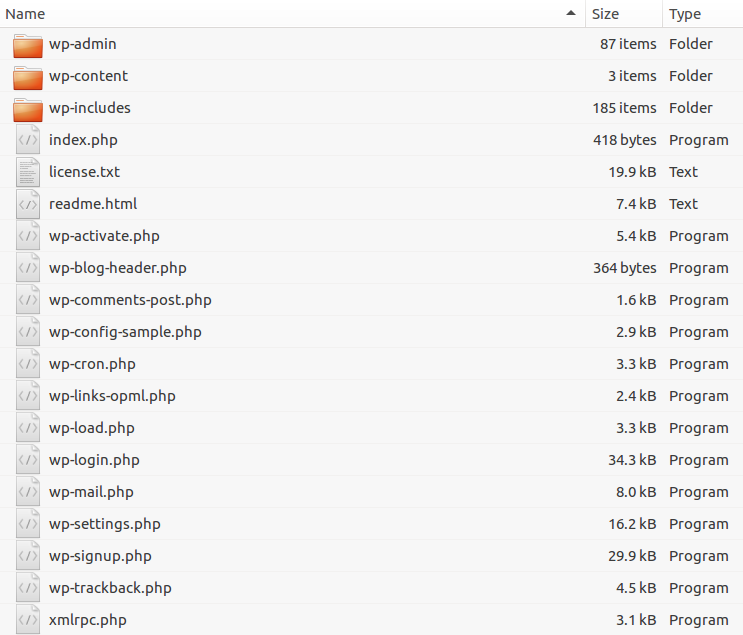
\includegraphics[width=\textwidth]{figure/wpfolder.png}
  \caption{Contenuto della cartella "wordpress".}
  \label{fig:wptree}
\end{figure}

\section{Creazione dello script di deploy}
Lo script di deploy, essendo tutte la macchine di sviluppo e produzione macchine Linux, è stato scritto in un file eseguibile
\emph{kirCMS-autodeploy.sh} utilizzando il linguaggio Bash ed utilizza una procedura simile allo script di deploy 
utilizzato da Kiruby.

Prima di eseguire il deploy è necessario fare commit sul master della repository di Wordpress in modo da avere i sorgenti git aggiornati.

Una volta committate le modifiche da pubblicare bisogna eseguire lo script \emph{kirCMS-autodeploy.sh} passandogli come argomento
\emph{lab} o \emph{pro} a seconda della macchina su cui si vuole deploiare.

Lo script per prima cosa chiede le credenziali di autenticazione, apre un tunnel verso la macchina dove si vuole deploiare, scarica l'ultima
versione zippata della repository e la invia alla macchina collegata.

Una volta collegato in remoto alla macchina su cui di deve deploiare, viene dezippata la repository e rinominata come \emph{wp-content}, mentre
quella che precedentemente si chiamava \emph{wp-content} viene rinominata \emph{wp-content-bkp} e quella che era \emph{wp-content-bkp}
viene cancellata.
Dentro\emph{wp-content} vengono eseguiti tutti i test di PhpUnit, eseguendo lo script presente all'interno della repository chiamato \emph{test.sh}.

Se i test falliscono viene stampato a console un messaggio con lo stack dell'errore, \emph{wp-content} viene cancellata e \emph{wp-content-bkp}
viene rinominata in \emph{wp-content}. In questo modo la procedura termina, lasciando online
la versione precedentemente pubblicata.

Se tutti i test passano invece la procedura termina e il server inizierà a
utilizzare le ultime modifiche.

La cartella \emph{wp-content-bkp} dove troviamo la precedente versione pubblicata serve a tenere quest'ultima ancora disponibile semplificando la precedura per un eventuale rollback. 

Se vengono individuati degli errori con il nuovo deploy, per ritornare alla situazione precedente è sufficente eliminare la cartella wp-content
e rinominare wp-content-bkp in wp-content.

\begin{verbatim}
	$ cd /media/www/wordpress 
	$ rm wp-content && mv wp-content-bkp wp-content
\end{verbatim}
\emph{comandi da eseguire a terminale per effettuare rollback alla versione precedente}

\newpage 

\begin{lstlisting}[language=bash,caption={Script di deploy: kirCMS-autodeploy.sh}]
#!/bin/bash

set -e

RED_COLOR=`tput setaf 1`
GREEN_COLOR=`tput setaf 2`
RESET_COLOR=`tput sgr0`

CHECKOUT_DIR=wpkiruby
TARFILE=wpkiruby.tar.gz
TARGET_DIR=/media/www/wordpress
WP_CONTENT=wp-content
WP_CONTENT_BKP=wp-content-bkp
UPLOADS=wp-content/uploads

LOGFILE=/media/www/wordpress/wp-content/themes/basic/test/.log.txt
LOAD=/media/www/wordpress/wp-load.php
TESTS=/media/www/wordpress/wp-content/themes/basic/test/.



#CHIEDI USERNAME E CONTINUA DOPO AVER APERTO IL TUNNEL
if [ ! "$1" ]
then
    echo "${RED_COLOR}Dimmi dove vuoi deployare! LAB \
    o PRO?${RESET_COLOR}"
    exit
fi
echo -n "Username: "
read username
gnome-terminal -e "$1.sh $username" 2>&1 > /dev/null &
echo "${GREEN_COLOR}Tunnellizzati e premi un tasto \
per continuare${RESET_COLOR}"
read

#SCARICA LA REPO DA GIT, COMPRIME E MANDA DOVE APERTO IL TUNNEL
cd /tmp && git clone git@gitlab.p7intranet.it:wpkiruby.git

tar -czvf $TARFILE $CHECKOUT_DIR
scp -P 20059 /tmp/${TARFILE} root@localhost:${TARGET_DIR}

rm $TARFILE
rm -rf $CHECKOUT_DIR

echo "${GREEN_COLOR}=== ${TARFILE} copied in remote at \
${TARGET_DIR} ===${RESET_COLOR}"

echo "=== switch WP-CONTENT and create WP_CONTENT_BKP ==="
#COLLEGA AD HOST REMOTO
ssh -C -l root -p 20059 -o UserKnownHostsFile=/dev/null -o \
StrictHostKeyChecking=no -R 8765:192.168.254.140:22 localhost \ 
-i /home/xpuser/shoppydoo/kiruby/key.ssh -t << HERE
    #ESEGUE IN REMOTO
    cd /media/www/wordpress; bash --login
    tar -xzf ${TARFILE}
    [ -d $WP_CONTENT_BKP ] && rm -rf $WP_CONTENT_BKP
    rm ${TARFILE}
    mv $WP_CONTENT $WP_CONTENT_BKP && mv $CHECKOUT_DIR \
    $WP_CONTENT
    chmod 777 -R $UPLOADS
    #ESEGUE I TEST E STAMPA ESITO IN FILE DI LOG
    phpunit --bootstrap $LOAD $TESTS > $LOGFILE
    if grep -q 'OK (' $LOGFILE;
    then
        echo '${GREEN_COLOR}All tests passed!!;
    else
        echo '${RED_COLOR}Tests not passed!! :(';
        cat $LOGFILE; echo '${RESET_COLOR}';
        rm -rf $WP_CONTENT && mv $WP_CONTENT_BKP \
        $WP_CONTENT;    
    fi
HERE
    echo "${GREEN_COLOR} Success, CMS is online!${RESET_COLOR}"
\end{lstlisting}

\newpage
\begin{lstlisting}[language=bash,caption={Lo script test.sh per eseguire tutti i test nella cartella \emph{test} e stamparne l'esito in un file di log e a console.}]
#!/usr/bin/env bash
LOGFILE=/media/www/wordpress/wp-content/themes/basic/test/.log.txt
LOAD=/media/www/wordpress/wp-load.php
TESTS=/media/www/wordpress/wp-content/themes/basic/test/.

phpunit --bootstrap $LOAD $TESTS > $LOGFILE
cat $LOGFILE;
\end{lstlisting}
  
%-------------------------------------------------------------
%       WIDGET ORIGINI
%-------------------------------------------------------------

\mcchap{Widgets di Origini}{cap:w-o}

\newpage

% ---------------- Origini - Slider prodotti ----------------

\section{Origini - Slider prodotti}
Il Widget "Origini - Slider prodotti" visualizza un box contente
4 vini, con titolo, sottotitolo e link per "Scopri altro".

Il form permette di modificare i seguenti campi (riferirsi a Figure \ref{fig:oprod}):
\begin{itemize}
\item Sottotitolo: il testo "Le selezioni"
\item Titolo: il testo "I consigli del sommelier"
\item Ids prodotti: la lista degli ID dei prodotti da visualizzare separati da virgola
\item Link: l'URL a cui punta il tasto \emph{Scopri Altro}
\end{itemize}

\begin{figure}
  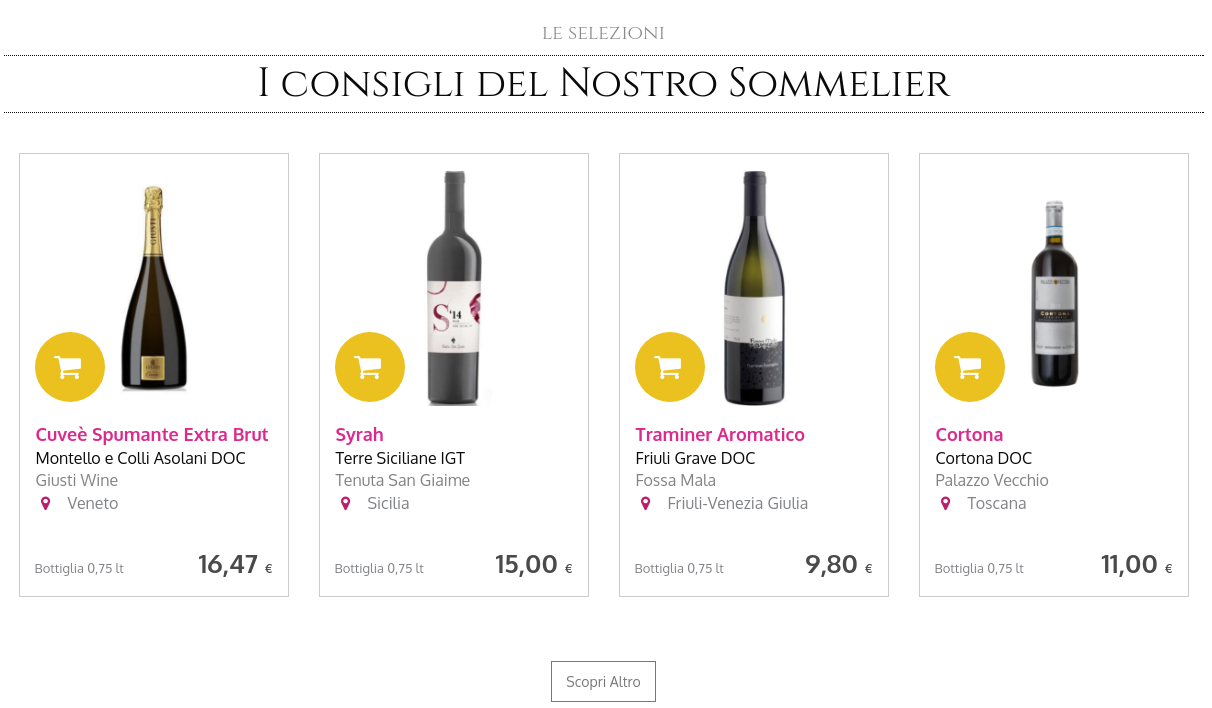
\includegraphics[width=\textwidth]{figure/oprod.png}
  \caption{Contenuto mostrato dal widget "Origni - Slider prodotti".}
  \label{fig:oprod}
\end{figure}


% ---------------- Origini - Banda tuttoschermo ----------------
\newpage
\section{Origini - Banda tuttoschermo}
Il Widget "Origini - Banda tuttoschermo" visualizza quella porzione di HTML
usata attualmente per lo "Speciale regione" (vedi Figure \ref{fig:oreg}).

Il form permette di modificare i seguenti campi (riferirsi a Figure \ref{fig:oreg}):
\begin{itemize}
\item Sottotitolo: il testo "Speciale regione"
\item Titolo: il testo "Lombardia e cultura del buon vino"
\item Descrizione: il testo della descrizione "La varietà dei territori..."
\item Link: l'URL a cui punta il tasto \emph{Scopri Altro}
\item Image-Link: l'URL dell'immagine di sfondo
\end{itemize}

\begin{figure}
  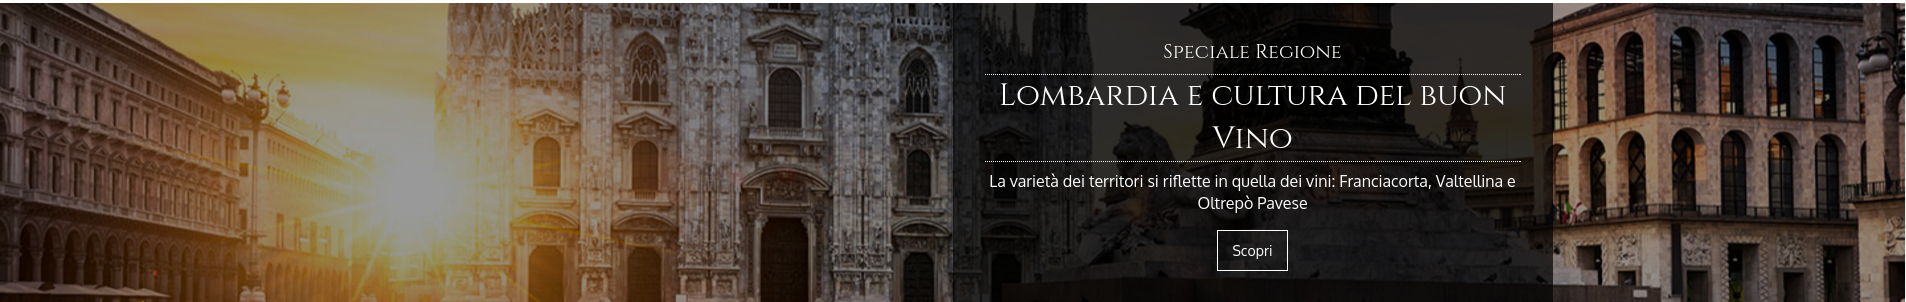
\includegraphics[width=\textwidth]{figure/oreg.png}
  \caption{Contenuto mostrato dal widget "Origni - Banda tuttoschermo".}
  \label{fig:oreg}
\end{figure}

% ---------------- Origini - Speciale ----------------
\newpage
\section{Origini - Speciale}
Il Widget "Origni - Speciale" visualizza quella porzione di HTML
usata attualmente per lo "Speciale del mese" (vedi Figure \ref{fig:ospec}).

Il form permette di modificare i seguenti campi (riferirsi a Figure \ref{fig:ospec}):
\begin{itemize}
\item Sottotitolo: il testo "La cantina del mese"
\item Titolo: il testo "Federico Ferrero"
\item Descrizione: il testo della descrizione "L’azienda agricola Ferrero nasce..."
\item Link: l'URL a cui punta il tasto \emph{Scopri Altro}
\item Image-Link: l'URL dell'immagine da visualizzare
\end{itemize}

\begin{figure}
  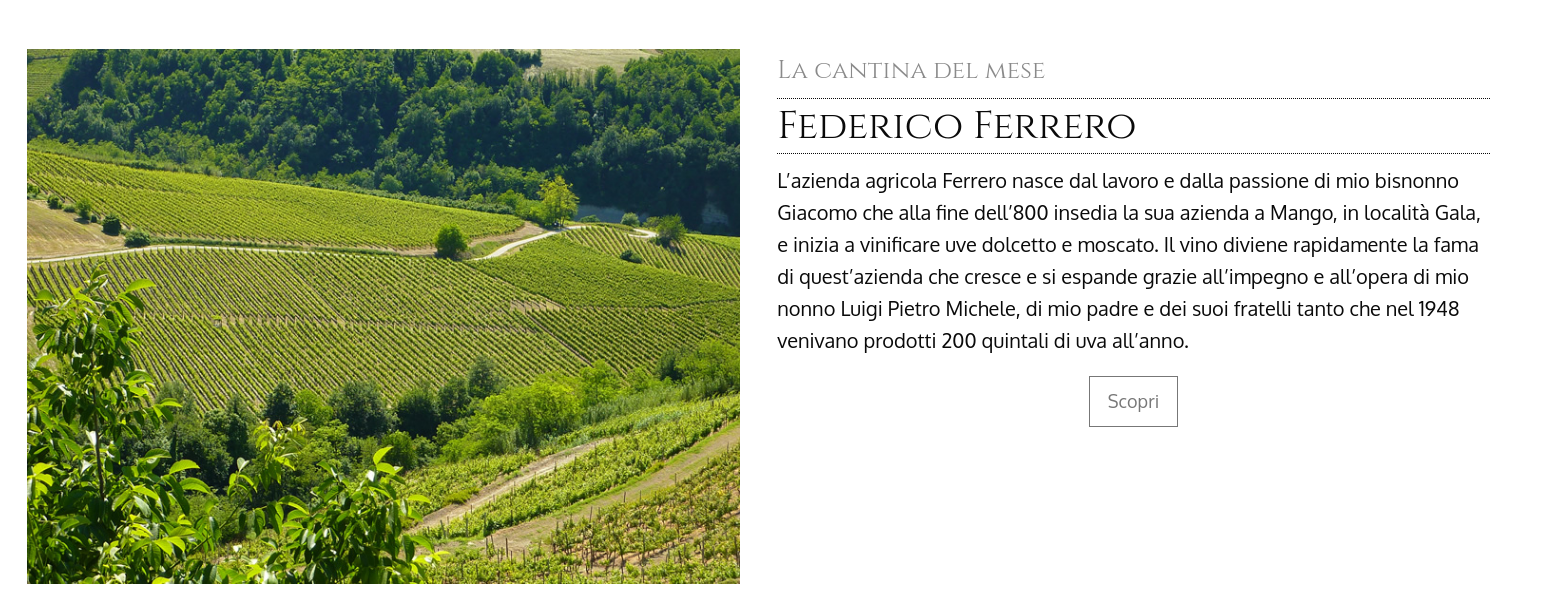
\includegraphics[width=\textwidth]{figure/ospec.png}
  \caption{Contenuto mostrato dal widget "Origni - Speciale".}
  \label{fig:ospec}
\end{figure}


  
%-------------------------------------------------------------
%       WIDGET ORIGINI
%-------------------------------------------------------------

\mcchap{Widgets di Kirivo}{cap:w-k}


%-------------------------------------------------------------
%       WIDGET KIRIVO
%-------------------------------------------------------------

\newpage

% ---------------- Kirivo - Immagini Speciali ----------------

\section{Kirivo - Immagini Speciali}

Il Widget "Kirivo - Immagini Speciali" permette di modificare il contenuto
delle prime due immagini della Homepage, ovvero le immagini solitamente dedicate
allo speciale del mese e alle offerte 

I campi che si possono modificare sono (riferirsi a Figura \ref{fig:kspec}):
\begin{itemize}
\item Link speciale: l'URL dove si viene indirizzati quando si schiaccia sull'immagine dello speciale
\item Url immagine speciale desktop: l'url dell'immagine da mettere nello speciale per desktop
\item Url immagine speciale mobile: l'url dell'immagine da mettere nello speciale per mobile
\item Link offerte: l'URL dove si viene indirizzati quando si schiaccia sull'immagine delle offerte
\item Url offerte speciale desktop: l'url dell'immagine da mettere nelle offerte per desktop
\item Url offerte speciale mobile: l'url dell'immagine da mettere nelle offerte per mobile
\end{itemize}

\begin{figure}
  
\includegraphics[width=\textwidth]{figure/kspec.png}
  \caption{Contenuto mostrato dal widget "Kirivo - Immagini Speciali".}
  \label{fig:kspec}
\end{figure}

% ---------------- Kirivo - Immagini Newsletter ----------------

\newpage
\section{Kirivo - Immagini Newsletter}

Il Widget "Kirivo - Immagini Newsletter" permette di modificare il contenuto
delle prime due immagini della Homepage, ovvero le immagini solitamente dedicate
allo speciale del mese e alle offerte 

I campi che si possono modificare sono (riferirsi a Figura \ref{fig:knews}):
\begin{itemize}
\item Url immagine newsletter desktop: l'url dell'immagine da mettere nella sezione "iscriviti alla newsletter"
\item Url immagine newsletter mobile: l'url dell'immagine da mettere nella sezione "iscriviti alla newsletter"
\item Link offerta: l'URL dove si viene indirizzati quando si schiaccia sull'immagine dell'offerta
\item Url offerta desktop: l'url dell'immagine da mettere nelle offerta per desktop
\item Url offerta mobile: l'url dell'immagine da mettere nelle offerta per mobile
\end{itemize}

\begin{figure}
  
\includegraphics[width=\textwidth]{figure/knews.png}
  \caption{Contenuto mostrato dal widget "Kirivo - Immagini Newsletter".}
  \label{fig:knews}
\end{figure}

% ---------------- Kirivo - Prodotti in evidenza ----------------

\newpage
\section{Kirivo - Prodotti in evidenza}

Il Widget "Kirivo - Prodotti in evidenza" visualizza quella porzione di HTML usata
per visualizzare i prodotti in evidenza (vedi Figura \ref{fig:kevid}).

I campi che si possono modificare sono (riferirsi a Figura \ref{fig:kevid}):
\begin{itemize}
\item Titolo: il testo "PRODOTTI IN EVIDENZA".
\item Ids: l'ID dei prodotti da visualizzare separati da virgola. I prodotti devono
essere almeno tre, se sono più di tre verranno usati i primi 3 ID validi.
\end{itemize}

\begin{figure}
  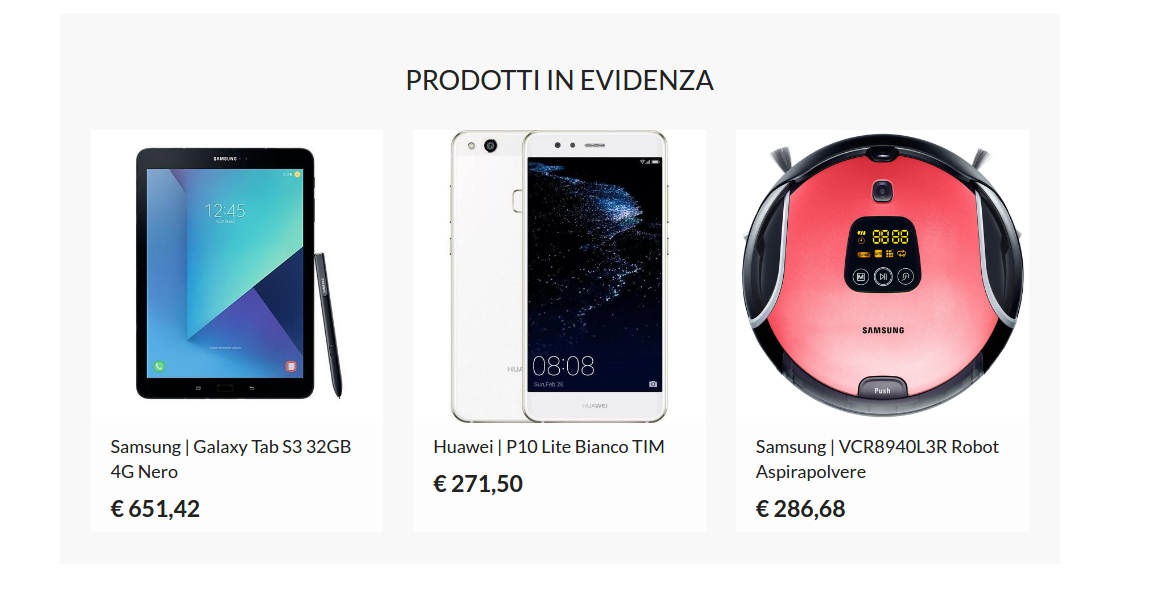
\includegraphics[width=\textwidth]{figure/kevid.png}
  \caption{Contenuto mostrato dal widget "Kirivo - Prodotti in evidenza".}
  \label{fig:kevid}
\end{figure}

\newpage
\section{Kirivo - Slider prodotti}

% ---------------- Kirivo - Slider prodotti ----------------

Il Widget "Kirivo - Slider prodotti"   visualizza quella porzione di HTML usata
per visualizzare uno slider di un insieme di prodotti (vedi Figura \ref{fig:kslide}).

I campi che si possono modificare sono (riferirsi a Figura \ref{fig:kslide}):
\begin{itemize}
\item Titolo: il testo "PRODOTTI PIÙ POPOLARI".
\item Numero max: il numero massimo di prodotti da visualizzare. Se lasciato vuoto non viene imposto alcun limite.
\item Ids: l'ID dei prodotti da visualizzare separati da virgola. I prodotti devono
essere almeno quanti specificati in numero max o quattro se non viene specificato.
\end{itemize}

\begin{figure}
  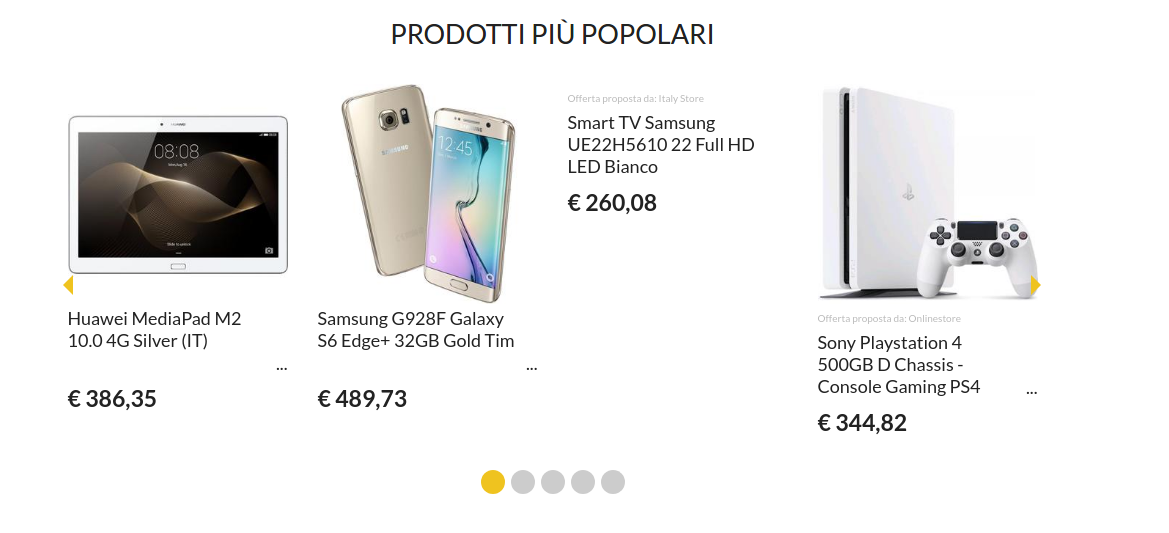
\includegraphics[width=\textwidth]{figure/kslide.png}
  \caption{Contenuto mostrato dal widget "Kirivo - Slider prodotti".}
  \label{fig:kslide}
\end{figure}


%%inserisci qui i tuoi capitoli
  
  \appendix
  %%%%%%%%%% CAPITOLO DI TESI %%%%%%%%%%
%
% Colophon 
%
%%%%%%%%%%%%%%%%%%%%%%%%%%%%%%%%%%%%%%
\chapter*{Colophon}

La tesi è stata scritta utilizzando il linguaggio LaTeX.\\
Le immagini sono state create appositamente usando screenshots delle applicazioni ed eventualmente editate con GIMP.\\


\backmatter{}

%% Bibliografia
  
  \printindex
  \bibliographystyle{bibliografia/IEEEtran}
  \bibliography{bibliografia/IEEEabrv,bibliografia/biblio}
   
\end{document}
